\documentclass[a4paper,11pt]{article}

% ConfigStream project report. The substantive paper body is embedded below
% so this file is a self-contained report entry point.
\usepackage[a4paper,margin=2.5cm]{geometry}
\usepackage{setspace}
\usepackage{graphicx}
\usepackage{booktabs}
\usepackage{tabularx}
\usepackage{longtable}
\usepackage{xcolor}
\usepackage{fancyhdr}
\usepackage{tikz}
\usetikzlibrary{calc}
% Keep hyperlinks when the local TeX installation has the full hyperref
% dependency set. The conditional fallback permits an offline PDF build on
% teaching-lab MiKTeX installations that omit stringenc.sty.
\IfFileExists{stringenc.sty}{\usepackage[hidelinks]{hyperref}}{\providecommand{\hypersetup}[1]{}}
\usepackage{natbib}

\onehalfspacing
\setlength{\parindent}{0pt}
\setlength{\parskip}{0.35em}

\definecolor{ConfigBlue}{RGB}{0,56,101}
\definecolor{ConfigRed}{RGB}{194,31,48}
\definecolor{ConfigGold}{RGB}{190,145,50}
\hypersetup{
    colorlinks=true,
    linkcolor=ConfigBlue,
    urlcolor=ConfigBlue,
    citecolor=ConfigBlue,
    pdftitle={ConfigStream Project Report},
    pdfauthor={Nguyen Duc Dung; Pham Cong Hoang; Mai Vu Hoang; Le Tien Hop}
}

\pagestyle{fancy}
\fancyhf{}
\fancyhead[L]{\small\textbf{ConfigStream}}
\fancyhead[R]{\small\textbf{Project Report}}
\fancyfoot[C]{\thepage}
\setlength{\headheight}{15pt}

\begin{document}

\begin{titlepage}
\thispagestyle{empty}
\begin{tikzpicture}[remember picture,overlay]
  \draw[ConfigBlue,line width=2pt] ($(current page.north west)+(0.75cm,-0.75cm)$) rectangle ($(current page.south east)+(-0.75cm,0.75cm)$);
  \draw[ConfigGold,line width=0.8pt] ($(current page.north west)+(0.92cm,-0.92cm)$) rectangle ($(current page.south east)+(-0.92cm,0.92cm)$);
  \draw[ConfigGold,line width=2pt] ($(current page.north west)+(0.75cm,-1.55cm)$) -- ($(current page.north west)+(0.75cm,-0.75cm)$) -- ($(current page.north west)+(1.55cm,-0.75cm)$);
  \draw[ConfigGold,line width=2pt] ($(current page.north east)+(-1.55cm,-0.75cm)$) -- ($(current page.north east)+(-0.75cm,-0.75cm)$) -- ($(current page.north east)+(-0.75cm,-1.55cm)$);
  \draw[ConfigGold,line width=2pt] ($(current page.south west)+(0.75cm,1.55cm)$) -- ($(current page.south west)+(0.75cm,0.75cm)$) -- ($(current page.south west)+(1.55cm,0.75cm)$);
  \draw[ConfigGold,line width=2pt] ($(current page.south east)+(-1.55cm,0.75cm)$) -- ($(current page.south east)+(-0.75cm,0.75cm)$) -- ($(current page.south east)+(-0.75cm,1.55cm)$);
\end{tikzpicture}
\centering
\vspace*{1.25cm}
{\Large\color{ConfigBlue}\textbf{HANOI UNIVERSITY OF SCIENCE AND TECHNOLOGY}\par}
\vspace{0.12cm}
{\large\textbf{School of Information and Communication Technology}\par}
\vspace{0.22cm}
\begin{tikzpicture}\draw[ConfigGold,line width=1.2pt] (0,0)--(13.2,0);\fill[ConfigRed] (6.4,-.06) rectangle (6.8,.06);\end{tikzpicture}
\vspace{1.25cm}
{\fontsize{23}{28}\selectfont\color{ConfigBlue}\textbf{PROJECT REPORT}\par}
\vspace{0.22cm}{\color{ConfigGold}\rule{7cm}{1pt}\par}
\vspace{0.45cm}
{\fontsize{22}{27}\selectfont\color{ConfigBlue}\textbf{ConfigStream}\par}
\vspace{0.18cm}
\vspace{0.18cm}
{\large\textbf{Version-aware configuration history, durable storage, and reproducible analytics}\par}
\vspace{0.22cm}
{\small\color{ConfigBlue}\textbf{Evidence boundary: 25 October 2026}\par}
\vfill
\begin{minipage}{0.82\textwidth}\renewcommand{\arraystretch}{1.22}
\begin{tabularx}{\linewidth}{@{}>{\bfseries}l@{\hspace{0.6cm}}X@{}}
Supervisor: & PhD Tran Viet Trung \\
\end{tabularx}\end{minipage}
\vspace{0.75cm}
\begin{minipage}{0.82\textwidth}\small
\begin{tabularx}{\linewidth}{@{}>{\bfseries}Xr@{}}\toprule
Member & \\\midrule
Nguyen Duc Dung & \\
Pham Cong Hoang & \\
Mai Vu Hoang & \\
Le Tien Hop & \\\bottomrule
\end{tabularx}\end{minipage}
\vfill
{\color{ConfigGold}\rule{5cm}{0.8pt}\par}\vspace{0.15cm}
{\large\color{ConfigBlue}\textbf{Ha Noi, 2026}\par}
\end{titlepage}

\pagenumbering{roman}
\tableofcontents
\clearpage

\listoftables
\clearpage

\listoffigures
\clearpage

\section*{List of Abbreviations}
\addcontentsline{toc}{section}{List of Abbreviations}
\begin{tabularx}{\textwidth}{@{}p{0.22\textwidth}X@{}}
    API & Application Programming Interface \\
    DNS & Domain Name System \\
    HA & High Availability \\
    IaC & Infrastructure as Code \\
    JSONL & JSON Lines \\
    RPKI & Resource Public Key Infrastructure \\
    RIS & Routing Information Service \\
    SQL & Structured Query Language \\
\end{tabularx}
\clearpage

\pagenumbering{arabic}

\clearpage
\section{Introduction}
ConfigStream is a Big Data platform for storing, comparing, and analysing configuration history. Its subject is an \emph{asset}: a router, NGINX/Linux host, application, or Kubernetes resource that owns a changing configuration. The platform is not an automated network-configuration framework and it is not a dashboard-first application. Its task is to turn source observations into a history that can answer, with evidence, which asset changed, between which versions, at which source time, under which normalization policy, and whether the answer can be reconstructed after a failure.

That task is harder than appending text files. A delivery can be retried, snapshots can arrive out of producer order, an event and its snapshot can be published to different Kafka topics without an atomic cross-topic relation, and a missing version can mean incomplete observation rather than deletion. Comparing the immediately preceding Kafka message with the current message is therefore not a history algorithm: it makes the meaning of a diff depend on transport order. Event-time systems expose lateness and state-retention choices \citep{AkidauEtAl2015Dataflow}; Kafka supplies a replayable partitioned log \citep{KrepsNarkhedeRao2011Kafka}; and Structured Streaming supplies incremental stateful execution \citep{ArmbrustEtAl2018StructuredStreaming}. ConfigStream composes these primitives with an application contract that separates source identity, version order, event time, and durable publication.

The platform has three input concepts. \texttt{Asset} identifies the durable logical subject. \texttt{ChangeEvent} records an independently observed event and may be related to a snapshot through metadata, but is not assumed to be atomically ordered with it. \texttt{ConfigSnapshot} is the versioned configuration observation used by the stateful diff path. The distinction prevents the report from treating every input as one kind of row. It also makes the evaluation honest: a Git history, a canonical RPKI member, a DNS measurement, and a RIS peer-prefix occurrence have different temporal semantics and must not be merged into one synthetic ``change rate.''

The central research question is: \emph{can a streaming data pipeline preserve a verifiable configuration history under disorder and replay while remaining recoverable and analytically useful?} We decompose it into three operational questions. RQ1 asks whether typed identities and bounded event-time state recover only justified adjacent producer-version transitions under retries and out-of-order delivery. RQ2 asks whether a lake-first commit boundary preserves authoritative history while allowing Elasticsearch, FastAPI, and dashboard views to be rebuilt. RQ3 asks how to evaluate correctness, throughput, storage, and resource cost without conflating workloads with incompatible units and completeness assumptions.

ConfigStream answers these questions through six implementation contributions. It defines versioned Pydantic contracts for assets, snapshots, events, diffs, alerts, and diagnostics; generates deterministic controlled workloads; implements identity-aware Spark state keyed by \texttt{asset\_id}; applies conservative text normalization and deterministic line diffs; commits raw provenance and typed outputs to manifest-backed Parquet before derived serving projections; and evaluates results with exact identity oracles, invariants, replay evidence, and explicit negative findings. The contribution is the composition of these boundaries into one inspectable pipeline, not a claim to invent Kafka, Spark, a temporal database, or a universally correct configuration parser.

The scope is intentionally bounded. Kafka is currently a local single-broker development topology; alert delivery can remain at-least-once; Spark measurements are often local; Elasticsearch is derived rather than authoritative; and observed histories are source-scoped proxies rather than direct deployment-frequency measurements. These restrictions are not footnotes. They determine which claims the experiments may support and which claims remain future work.

\section{Related Work and Background}
\subsection{Processing models}
MapReduce, Spark, Kafka, and Structured Streaming provide the primitives for distributed batch and stream processing \citep{DeanGhemawat2004MapReduce,ZahariaEtAl2012RDD,KrepsNarkhedeRao2011Kafka,ArmbrustEtAl2018StructuredStreaming}. The Dataflow Model explains why event-time, watermarks, and out-of-order input must be explicit correctness and cost choices \citep{AkidauEtAl2015Dataflow}. ConfigStream places an application-specific state contract on top of those components: asset identity and producer version define adjacency.

\subsection{Configuration and storage}
Git, Oxidized, Puppet, Batfish, and gNMI address versioning, collection, desired-state management, semantic validation, and protocol access. ConfigStream is not a replacement for these systems. It preserves raw content and hashes, applies a conservative normalization policy, and computes a deterministic line diff. Delta Lake motivates reliable object-store commit boundaries, while DuckDB motivates a strong local analytical baseline \citep{ArmbrustEtAl2020Delta,RaasveldtMuhleisen2019DuckDB}.

\section{Methodology}
\label{sec:platform-method}

ConfigStream is organised around one principle: a derived temporal statement is valid only when its identity, source coordinate, ordering semantics, provenance, and publication boundary are explicit. The repository therefore contains a common evidence layer and several workload-specific paths. The common layer supplies typed contracts, deterministic identities, source manifests, lake commits, reconciliation, and reproducible evaluation. It does not force all sources into one temporal model. Configuration snapshots are versioned states; RPKI is a complete daily authorization state; RIS is a stream of peer-prefix occurrences; DNS is a set of observations with explicit uncertainty. Treating these as interchangeable rows would make subsequent analytics easy to code but scientifically ambiguous.

\subsection{Common evidence contract}

Every temporal record has a logical identity and a provenance binding. The temporal schema package defines envelopes, source manifests, artifacts, time descriptors, source coordinates, and record kinds. Logical identities are generated from canonical bytes under a named policy, rather than from a database auto-increment or a message offset. Source manifests record source identifier, dataset identifier, scope, artifact inventory, hashes, and acquisition metadata. A consumer can consequently distinguish a repeated delivery of the same logical record from a conflicting record that merely has similar content.

This contract is deliberately stronger than a data-frame schema. A data frame can contain a date column without establishing that a record is complete for that date, or contain a SHA-256 without stating which source artifact it hashes. ConfigStream stores these relationships as first-class fields because a historical state or transition must be explainable after the job that created it has finished. The contract also separates known time, unknown time, and intervals. An absent timestamp is not silently converted into an arbitrary timestamp merely to make a window query run.

\subsection{Configuration-history path}

The configuration path begins with assets, independent change events, and configuration snapshots. Kafka topics are intentionally distinct: \texttt{config.assets} is compacted; \texttt{config.events}, \texttt{config.snapshots}, and \texttt{config.alerts} have their own partitioning and delivery behavior. Spark's stateful configuration query consumes the snapshot topic because snapshots are the records from which a version-adjacent textual transition can be justified. Events may be associated by metadata, but the code makes no cross-topic atomic-ordering claim.

The first stateful processor binds snapshot identity. The second stores a bounded, version-sorted buffer per \texttt{asset\_id}. A candidate can be rejected as an exact retry, snapshot-identity conflict, version conflict, or evicted version. For an accepted candidate, the pure transition emits a pair only when the successor producer version equals the predecessor version plus one. The code-backed teaching example is an arrival sequence of v1, v3, and v2: no v1--v3 edge is created while v2 is absent; when v2 arrives within retention, v1--v2 and v2--v3 are emitted. These labels are illustrative integer versions, not fixed values in the implementation. Watermark delay, timeout, buffer cap, eviction floor, and emitted-edge flags bound the claim.

Each eligible pair is normalized under a named conservative text policy, compared with deterministic line-based logic, and passed to validated YAML rules. The raw hash remains evidence about source bytes; the normalized hash is evidence about the supported canonical text. The two must not be conflated. Rules operate on normalized diff lines and create deterministic alert identities, but they do not prove semantic deployment safety or exactly-once external alert delivery.

\subsection{RPKI complete-state and transition path}

RPKI is not processed through the configuration version buffer. The dedicated RPKI Spark path decodes source chunks into source rows, validates row payload digests, reconciles retries by row identity, and writes a raw source ledger. A daily state is publishable only after the implementation has observed the complete expected row-index inventory, verified source provenance and artifact hash, compared the source coordinate map with an independent oracle, deduplicated canonical members, and checked the resulting member count and state digest against the observation descriptor.

The output of this path is a complete authorization-member state, not a sequence of configuration lines. A daily transition is valid only when the two day references are consecutive, compatible under their comparison and validation policies, and backed by verified complete endpoint states. This is why RPKI storage and query results can support statements about added or removed authorization members, whereas an incomplete arbitrary Kafka window cannot. The code rejects a partial day rather than inferring a state from the rows observed so far.

\subsection{RIS occurrence path}

The RIS path reads MRT archives through bounded framing, decodes route records, and projects them into native peer-prefix occurrences. Occurrence identity preserves the source frame and record coordinate; repeated occurrences are not automatically duplicates. This choice protects multiplicity: a collector can observe the same prefix through different peers or at different records, and collapsing them into a set would answer a different question. Historical closure and reconciliation are therefore defined over declared occurrence identities and source coordinates, not over an assumed complete global routing table.

The report consequently uses RIS for occurrence-processing, framing, temporal-window, and recovery evidence. It does not claim that a RIS input is a complete BGP state or that a count of occurrences is the number of unique deployed routes. Queries and analytics make their time-window and prefix/peer filters explicit, and provenance can be traced back to the frame-level source coordinate.

\subsection{DNS observation path}

The DNS path is a measurement path with a different uncertainty model. Raw selected-address records are committed first; grouping canonicalises query and response names, collects address and worker sets, records minimum and maximum known timestamps, and flags unknown worker or time values. A qualified comparison must account for source completeness and vantage conditions. In particular, absence in an incomplete or unverified observation is not converted into a strong claim that a DNS answer disappeared globally.

This design prevents an attractive but invalid generalisation: treating DNS records as versioned configuration states. The code can calculate a difference between qualified observations under a declared policy, but it retains uncertainty fields in the output. DNS therefore contributes evidence about robust temporal processing of measurements, not proof of a global authoritative DNS history.

\subsection{Publication, reconciliation, and analytics}

The configuration stream writes raw and processed Parquet datasets by query and batch before optional search indexing and alert publication. Its manifest records counts, paths, and an inventory of Parquet files with byte lengths and SHA-256. On replay, the writer validates the prior manifest and compares the expected and committed logical projection. The temporal typed-publication foundation applies the same idea to registered temporal record kinds: it reconciles records against their manifests, validates any required complete input state, hashes the canonical logical projection, and stores a typed commit containing record kind, dataset path, provenance identifiers, and digest.

Analytics runs only over committed Parquet. It loads and validates committed inputs, reconciles history by the appropriate deterministic identity, omits sensitive normalized-content/details fields from analytical inputs, and writes a separately validated analytical commit. Elasticsearch and FastAPI are serving projections. They are useful for pagination, lookup, latest-version queries, and aggregates, but neither changes what was committed nor becomes the source of truth. If indexing fails after the lake commit, the appropriate recovery is reindexing from the committed lake projection.

\subsection{Evaluation methodology}

Evaluation follows the same source-specific semantics. Synthetic configuration workloads make disorder, retry, mutation, and version adjacency controllable. Observed Git histories provide source-scoped configuration-evolution proxies. TerraDS supplies a separate replay corpus. RPKI compares complete canonical-member states and selected representation layouts. RIS measures framed occurrence processing. DNS evaluates measurements while retaining completeness and vantage qualifiers. The primary correctness oracle is an exact identity-to-full-record projection wherever one is available; counts, hashes, and schema reads are supplementary integrity checks.

Performance measurements declare their processing boundary and unit. The matched B0/B2/B3 campaign fixes one normalized output projection before comparing local, Spark batch, and queued streaming execution; it is not a claim about all source-acquisition or production-recovery costs. End-to-end replay includes Kafka, state, lake, and drain, and therefore reports different denominators. Results are accepted only when the registered projection and resource rules hold. Failed, invalid, and not-run cells remain visible instead of being converted into successful averages.

\section{Architecture Interpretation}
\label{sec:architecture-interpretation}

Figure~\ref{fig:architecture} should be read as an evidence architecture, not as a generic left-to-right technology stack. The upper configuration lane produces stateful version-adjacent diffs and rule alerts. The lower temporal lanes preserve their own object semantics and publish typed evidence. Both lanes meet only at the committed lake and the analytics/reconciliation layer. The figure must not draw an arrow that suggests RPKI, RIS, or DNS flow through the configuration normalizer or version buffer; that would be false according to the implementation.

The authoritative boundary is the commit manifest, not Kafka and not Elasticsearch. Kafka is the replayable transport for the relevant paths. Elasticsearch and the API are read projections. This placement explains why a durable committed record can coexist with an incomplete dashboard and why repair proceeds from Parquet rather than from whichever service responded last.

\clearpage
The methodology is organized around a precise state transition rather than around the deployment components. A valid transition has four requirements: both records refer to the same asset, the producer versions are consecutive in the retained history, the records pass the snapshot contract, and the resulting diff can be traced to a committed run. Arrival order is treated as delivery metadata, not as the meaning of configuration history.

\begin{figure}[t]
\centering
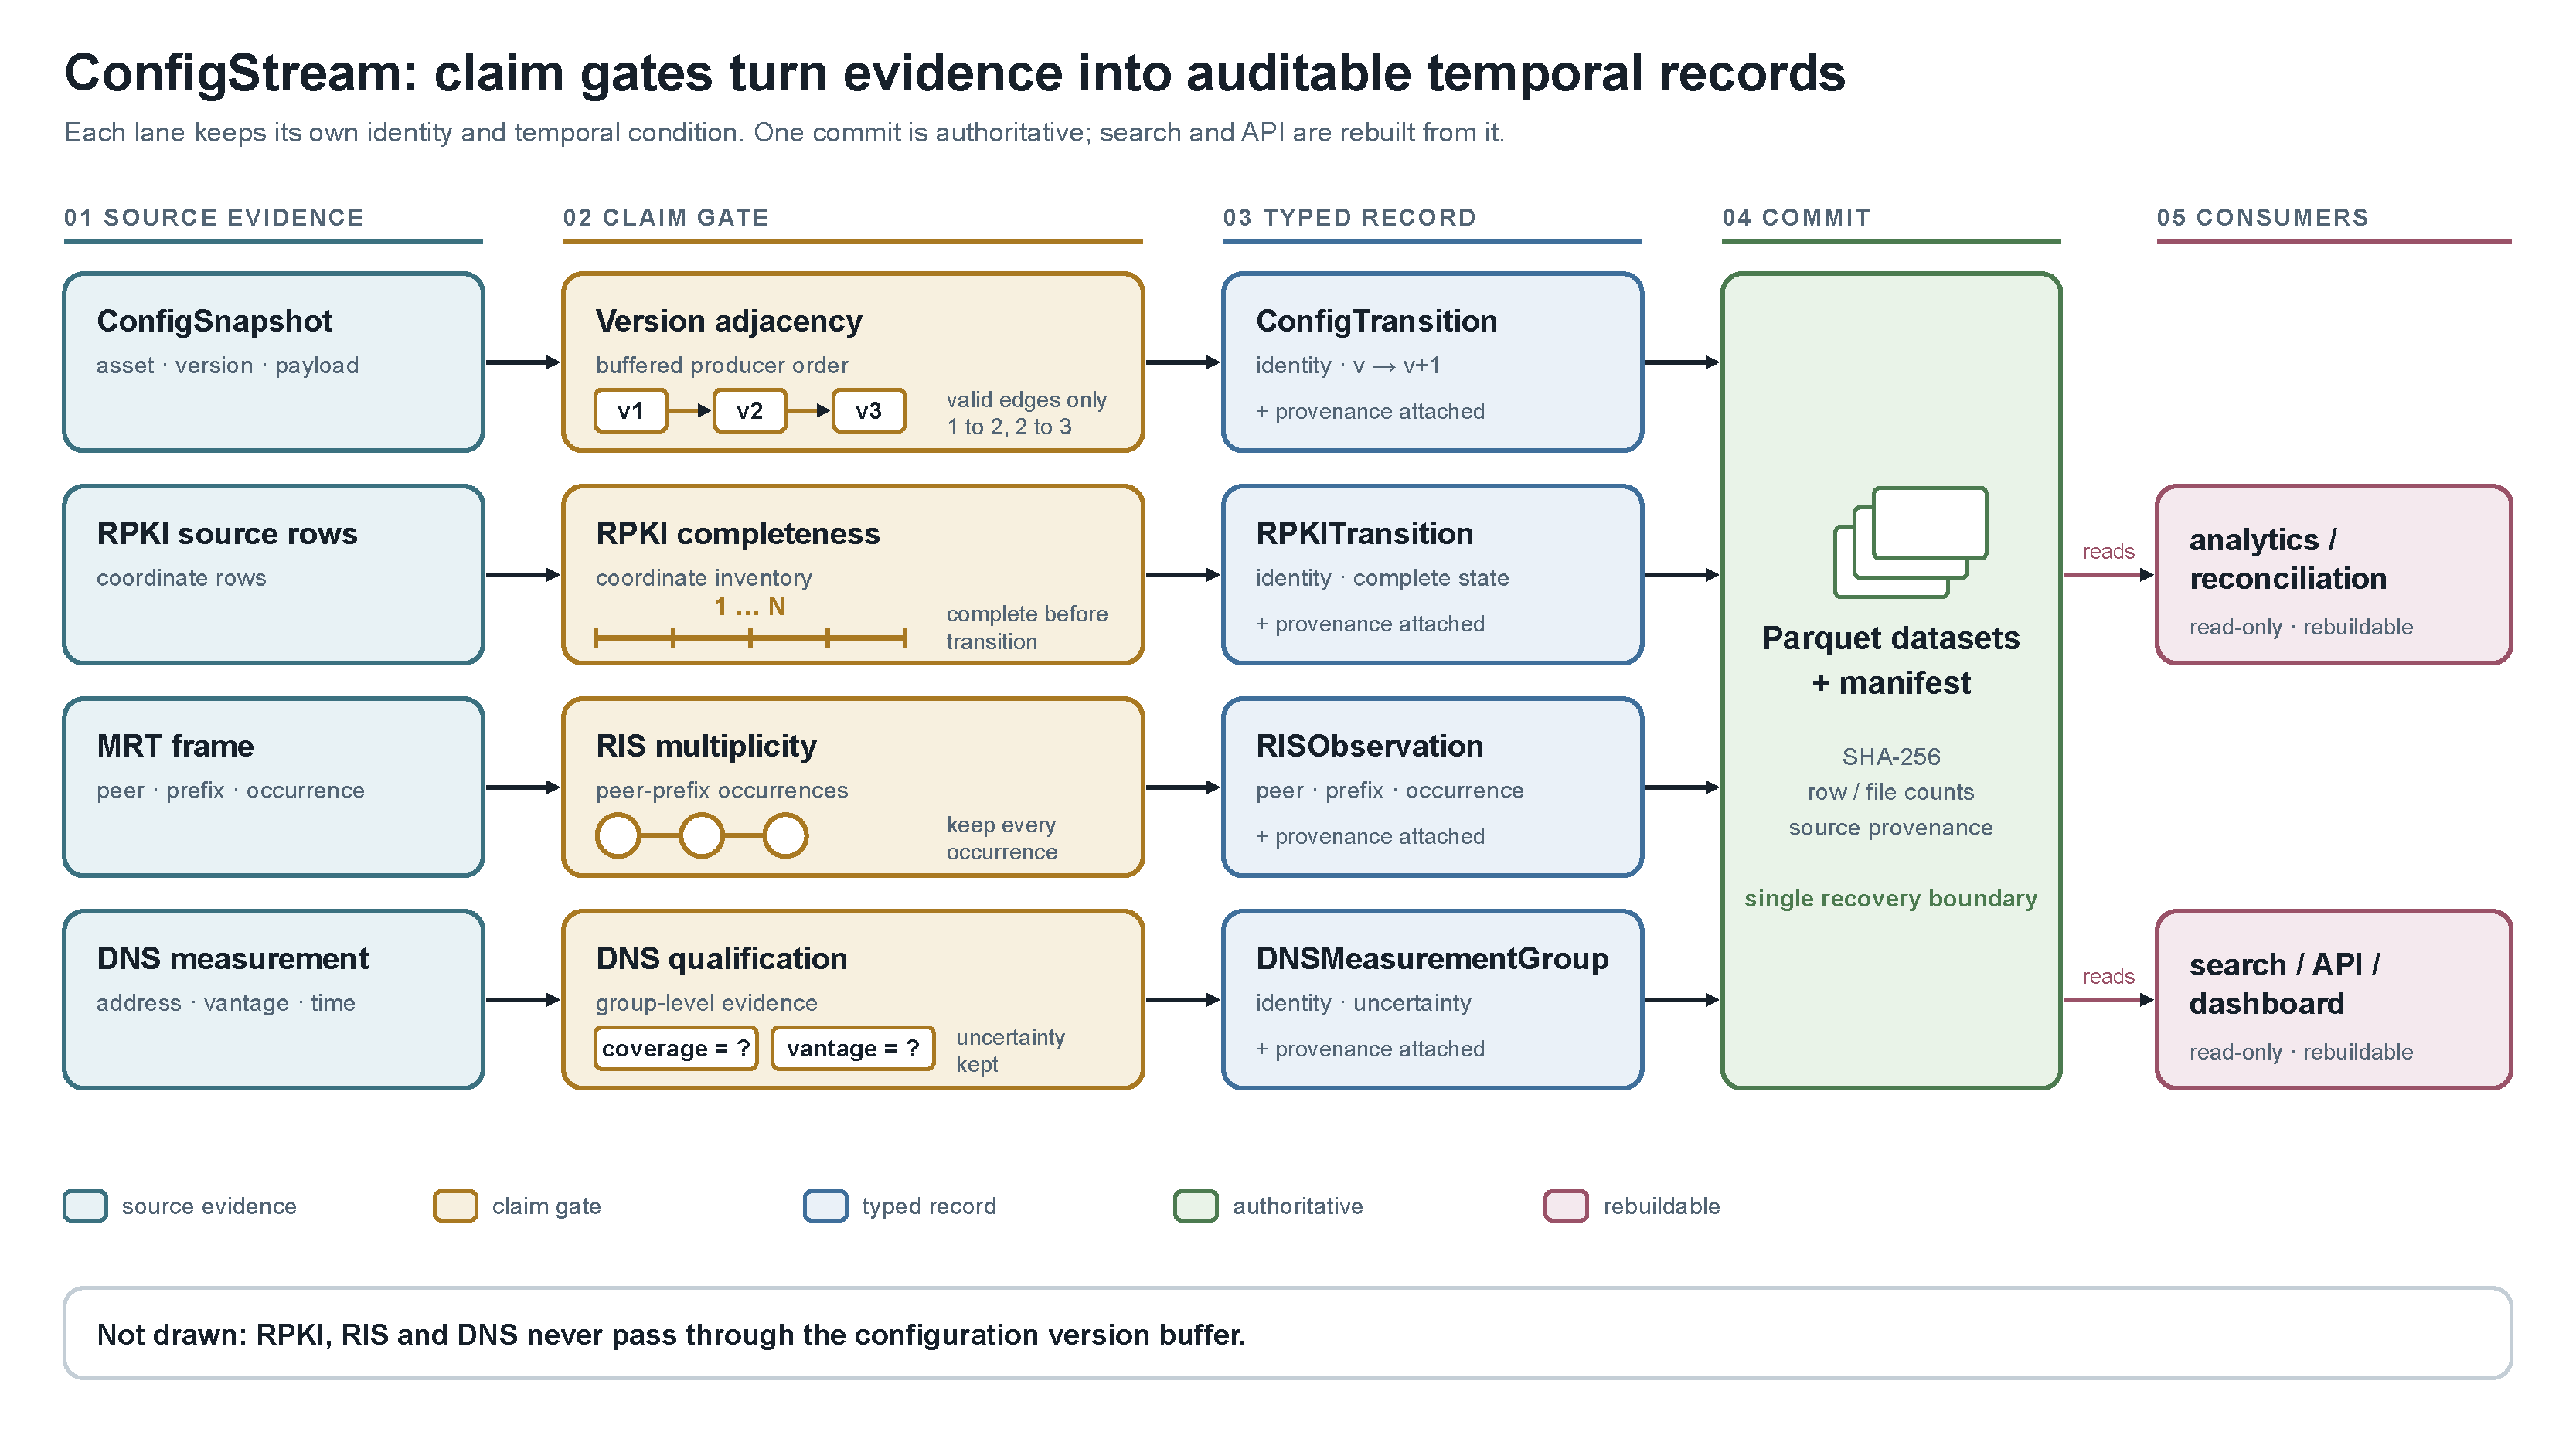
\includegraphics[width=\linewidth]{figures/configstream-platform-architecture.pdf}
\caption{ConfigStream's evidence path. Typed snapshots enter the stateful processor; the processor orders retained versions by producer version, emits only justified adjacent edges, computes a deterministic semantic diff, and commits one manifest that separates authoritative Parquet history from rebuildable serving projections. Evaluation reads the same run evidence and reports correctness, cost, and diagnostics with their workload units.}
\label{fig:architecture}
\end{figure}

\subsection{Contracts and admission}
ConfigStream keeps asset, snapshot, event, diff, alert, and diagnostic as separate contracts. A snapshot contains an asset identifier, an immutable snapshot identifier, a producer version, event time, ingest time, a content location, and a raw SHA-256. The contract checks local shape and content integrity. It does not claim that a record is globally unique, that Kafka delivery is ordered across topics, or that cross-topic writes are atomic.

Admission begins by binding the snapshot identifier to its source identity. An exact retained retry is suppressed. A conflicting binding produces a source-identity diagnostic. If a retained asset already contains the same version with another snapshot identifier, the first accepted version wins and the conflicting record is reported as a version conflict. Versions at or below the capacity-eviction floor are rejected as evicted history. These checks happen before normalization and prevent malformed or contradictory records from silently changing the state.

\subsection{Event-time state and latest-version semantics}
One Spark Structured Streaming query consumes \texttt{config.snapshots}. The query validates records, applies an event-time watermark, performs bounded identity deduplication, groups records by \texttt{asset\_id}, and invokes native per-key state. The state contains a bounded list of accepted versions, an eviction floor, emitted-edge flags, and an event-time inactivity timer. The default policy retains at most 32 versions per asset, uses a 10-minute watermark delay, and expires inactive asset state after 30 minutes of event time.

The state buffer is sorted by producer version, not by Kafka offset, arrival order, or timestamp order. The latest snapshot is therefore the retained accepted record with the maximum producer version. In the running out-of-order example, the accepted versions are v1, v2, and v3, although they arrive as v1, v3, v2. The system keeps the history in version order and reports v3 as the latest snapshot after the buffer is complete.

This distinction is important. The processor does not compare v1 directly with v3 merely because v2 has not arrived yet. It waits while the relevant history remains retainable. Once v2 arrives, it can emit the two justified edges v1 to v2 and v2 to v3. If a missing endpoint is evicted or the asset times out, the system emits a bounded gap or eviction diagnostic. It does not invent a replacement transition. A first observation of v3 also produces no baseline diff; an earlier retained version can complete the edge later.

\subsection{Adjacent-edge construction}
For each newly admitted snapshot, the processor inserts the record into the version-sorted buffer. It then examines neighboring versions whose edge flag is not set. An edge is eligible only when the two endpoints are consecutive in the version sequence accepted for that asset. After a successful comparison, the edge flag prevents replay of the same logical transition from producing another logical diff.

This policy explains the difference between the online and offline paths. The offline pair API may compare two explicitly supplied versions and reports a version gap when they are not consecutive. The streaming path is stricter because it must infer transitions from an incomplete, reordered history. It emits an edge only when the predecessor and successor are justified by the retained state. State eviction and timeout deliberately bound how much late history can be repaired.

\subsection{Normalization, diff, and rules}
For each eligible edge, ConfigStream reconstructs the two supported inline text snapshots and applies the Phase 5 normalization policy exactly once. The policy canonicalizes line endings, removes selected generated comments and trailing whitespace, canonicalizes selected separators, and masks selected secret-like values. It is deterministic and idempotent for the supported representation. The raw hash and normalized hash remain separate, so a source-byte change can be distinguished from a change that survives normalization.

The normalized contents are compared with the deterministic line-diff implementation. YAML rules are validated at application startup and matched against normalized diff lines. An alert records the new snapshot identifier, event time, rule identifier, severity, and a deterministic alert identifier. The implementation is deliberately narrower than a universal configuration parser or a universal secret detector. Unsupported content locations, unsafe syntax, or model failures become safe processing diagnostics rather than silently accepted diffs.

\subsection{Commit boundary and serving projections}
The output boundary is implemented as one \texttt{foreachBatch} path. A complete accepted batch is written to the committed Parquet history in MinIO before optional metadata indexing and alert publication proceed. The commit manifest records source identifiers, row counts, hashes, and batch-level provenance. Parquet is therefore the authoritative recovery path. Elasticsearch, FastAPI, and the dashboard expose safe metadata and aggregate views that can be rebuilt from committed history.

This is a recovery contract, not an atomic transaction across all sinks. A search write can fail after Parquet commits, and a sink retry can produce physical Kafka duplicates. Deterministic identifiers support logical deduplication in serving storage, but they do not establish end-to-end exactly-once delivery. The architecture reports these limits explicitly because they affect how the experiment and the final claim must be interpreted.

\subsection{Evaluation design}
The evaluation uses four evidence roles. Versioned configuration tests whether asset identity and adjacent history are preserved. Complete state tests exact membership and transition reconstruction. Measurement workloads test bytes, wall time, lag, drain, and resource guards under declared denominators. Event workloads test occurrence multiplicity and diagnostics without treating repeated observations as one state.

For each accepted run, the evaluator compares complete identity-to-record projections against an independent oracle where available. Counts and checksums are secondary checks; they cannot replace membership comparison. The run manifest links the input scope, processing boundary, output artifacts, acceptance criteria, and negative findings. Rates are reported with their unit, such as snapshots per second, canonical rows per second, or occurrences per second. Unmeasured dimensions remain labelled as unmeasured.
\section{Experiments}

\subsection{Experimental questions and acceptance logic}
The experiments test properties that follow directly from the implementation. First, the stateful path must preserve version order when Kafka delivery does not. Second, committed lake data must be sufficient to validate a replayed batch and to support rebuildable read projections. Third, performance comparisons must hold the output projection fixed before comparing execution time. A run is accepted only after its output projection satisfies the registered exactness rule. A successful wall-clock measurement without an exact projection is not counted as a result.

The implementation exposes three useful correctness boundaries. The in-memory transition tests exercise the version buffer, edge flags, eviction floor, and timer behaviour without a transport. The Spark tests exercise the native \texttt{transformWithStateInPandas} state store and checkpoint behaviour. The integration path exercises Kafka ingestion, stateful processing, lake publication, and read-only retrieval. This separation matters: an error in pair selection, a failed Parquet commit, and a failed metadata projection are different failures and should not be collapsed into one pass/fail label.

\subsection{Workloads, units, and compared systems}
The configuration-history workload uses the accepted TerraDS history: 6,505 file incarnations, 10,188 versions, 3,683 ordinal adjacent edges, and 12,278,085 UTF-8 bytes. Each file history is ordered by its accepted version/ordinal relation. The RPKI, DNS, and RIS workloads are retained as distinct evidence roles. RPKI uses canonical authorization members, DNS uses raw measurements and qualified address-group comparison, and RIS uses native peer-prefix occurrences. These objects have different semantics, so a rate in files/s, rows/s, or occurrences/s is never aggregated into a single system-capacity number.

The matched normalized-core campaign compares three execution modes over the same complete output projection: B0 is a direct Arrow-based local rewrite, B2 is a Spark batch rewrite, and B3 is a queued Spark streaming rewrite. Each mode receives the same retained normalized input, produces the same logical rows, and is checked against the same independent projection. The comparison intentionally excludes parser construction, source acquisition, and production-specific state/group finalization in every mode. It therefore measures a controlled processing boundary, not the cost of a full deployed service.

\subsection{Correctness protocol}
The primary oracle is an identity-to-full-record comparison. For every accepted output, the evaluator checks missing identities, extra identities, conflicting identities, duplicate identities, and complete row equality. Counts, digests, and selected offsets are secondary evidence. The protocol matches the code's own failure model: a version conflict, an evicted predecessor, or a state timeout yields a diagnostic instead of a fabricated transition.

For the version-state path, the decisive adversarial case is an out-of-order history. The processor accepts v1, v3, and v2 for one asset, keeps the records sorted as v1, v2, v3, and emits only v1 to v2 and v2 to v3. The maximum retained version, v3, is the current/latest accepted state for that asset. The API independently sorts snapshot documents by version descending and then snapshot identifier ascending; its latest endpoint therefore does not depend on ingest order. Tests cover duplicate replay, version conflict, missing versions, buffer eviction, state expiry, and restart boundaries.

For committed lake data, the writer partitions each emitted record type, writes Parquet, inventories every Parquet file with its byte length and SHA-256, rereads the data under the expected schema, and verifies physical row counts before writing the manifest. On replay of an existing batch, the writer compares the expected projection with the committed projection before preserving the existing files. This is stronger than merely checking that a directory exists, but it remains a local commit protocol rather than an all-sink transaction.

\subsection{End-to-end replay result}
The accepted TerraDS replay processed 10,188 snapshots and formed 3,683 adjacent diffs. It committed 29,402,997 bytes of raw and processed Parquet data, emitted zero alerts and zero diagnostics, and completed in 68.742 seconds including drain. The source-side publisher rate was 500.023 snapshots/s; the separately defined accepted logical rate was 148.205 snapshots/s. These measures describe different boundaries and are reported separately.

The replay supports a limited but useful conclusion. Under the retained history and local deployment, ConfigStream reconstructed every accepted adjacent edge through Kafka, native Spark state, and the lake sink without producing a false alert or a recorded state diagnostic. It does not show that every sparse production history can be repaired after a long inactivity gap, because the implemented state has an inactivity timeout and a bounded version cap.

\subsection{Matched processing result}
The corrected campaign contains 27 successful trials: three fresh-process repetitions for each workload/mode combination. Every trial matched the complete independent normalized projection. All nine B3 trials ended with zero selected-offset lag. Table~\ref{tab:timing} reports the median command-start-to-observed-exit time; the ranges show run-to-run variation rather than a statistical confidence interval.

\begin{table}[t]
\centering
\caption{Matched normalized-core execution time in seconds. Every cell has three exact-output repetitions.}
\label{tab:timing}
\small
\begin{tabular}{lccc}
\toprule
Selected unit & B0 & B2 & B3 \\
\midrule
RPKI, 360,226 members & 6.297 (6.282--12.577) & 16.840 (14.729--21.080) & 25.417 (23.144--25.424) \\
RIS, 370,141 occurrences & 10.485 (8.437--12.636) & 21.167 (18.967--23.186) & 29.644 (23.233--29.726) \\
DNS, 4,096 measurements & 2.089 (2.087--6.302) & 10.536 (10.486--12.584) & 16.866 (12.624--16.924) \\
\bottomrule
\end{tabular}
\end{table}

B0 is faster than B2, which is faster than B3 within this registered boundary. That ordering is compatible with the additional Spark startup, scheduling, and queued-publication work in B2 and B3, but it is not a general ranking of the complete systems. The trial does not include the parsing, long-lived state finalization, or full recovery work that a production deployment would incur.

\subsection{Storage representation result}
A separate RPKI representation experiment compares three exact, normalized analytical layouts. All registered queries returned exact outputs in the retained result artifact. R1 occupies 47,756,423 analytical bytes, R2 occupies 3,555,516 bytes, and R3 occupies 6,954,890 bytes. Relative to R1, R2 reduces the analytical footprint by 92.55\% and R3 by 85.44\%. Both R2 and R3 satisfy the registered requirement that every selected query remain within twice the R1 median time, so both are preferred within this local analytical policy.

This result must be read narrowly. The accounting refers to the declared analytical representation, not every source archive, cache, container image, object-store overhead, or production operational cost. It demonstrates that the chosen canonical representations can preserve the required RPKI projection while reducing the specified storage target; it does not establish a universal storage winner.

\subsection{Resource and negative-result boundary}
The corrected normalized-core campaign recorded 502.981 seconds across the retained initial attempt and approved retry, 3,869,485,576 bytes of retained growth, and a peak sampled process tree of 1,612,824,576 bytes. These remained below the amended 7,200-second and 6-GiB campaign limits. The initial attempt is retained separately because a SQLite connection was used from the wrong Spark callback thread. It committed zero batches. The corrected implementation serialized the cross-thread use and then completed the approved 27 trials; it is not legitimate to average the failed attempt into a success rate.

The unrun cases are also results about scope. The full paced RIS matrix was not executed, and no new physical 1x paced replay established its drain ratio. Consequently, the project does not claim streaming superiority, horizontal scalability, high availability, or an end-to-end exactly-once guarantee. Those claims require experiments beyond the measured local boundary.
\section{Discussion}
\subsection{What the system makes auditable}
The system makes four decisions inspectable. First, identity is visible in the record and is not reconstructed from a display row. Second, temporal order is derived from a producer version within an asset rather than from arrival order. Third, the durable boundary is visible in the commit manifest and Parquet inventory. Fourth, the evaluation preserves source role, oracle, denominator, and failure state. These decisions convert an opaque pipeline into a sequence of contracts that can be checked independently.

This matters for the meaning of a negative result. If a run is stopped before commit, the correct output is an uncommitted attempt, not a zero-row successful run. If a paced experiment is not authorized or not started, the correct label is \texttt{NOT\_RUN}, not an inferred capacity bound. If a simple batch baseline is faster on a bounded window, that is evidence about workload fit, not evidence that the streaming design is incorrect.

\subsection{Limitations and threats to validity}
The deployment topology is local or single-node. The Kafka broker uses replication factor one and loopback plaintext. The accepted evidence therefore does not establish high availability, distributed-cluster scalability, cloud object-store behavior, or end-to-end exactly-once delivery. Checkpoint recovery is tested within declared local boundaries; it is not a proof against every retention, host, or image failure.

The workloads are bounded and source-specific. Public Git history is a proxy for configuration evolution, not deployment frequency. RPKI, DNS, and RIS cover registered scopes and windows rather than entire infrastructures. The DNS role explicitly contains uncertainty about absence and observation conditions. The RIS role describes collector occurrences, not a complete routing state. These limits prevent a single cross-domain rate table from being scientifically meaningful.

The matched campaign excludes parsing and production state finalization in every mode. Filesystem cache temperature was not controlled as a cold-cache experiment. CPU, physical query I/O, and network wire bytes were not measured. The paper therefore reports the registered boundary and leaves broader performance questions open.

\subsection{Future work}
The next experiment should be the registered paced RIS replay, with the existing identity ledger and acceptance criteria unchanged. A second priority is an all-in matched comparison that includes source parsing, state/group finalization, publication, validation, and recovery. A third is controlled checkpoint fault injection, including interrupted writes and search rebuilds from committed Parquet. Each extension should retain the existing negative findings and should not replace an unexecuted cell with an older unmatched measurement.

% Shared implementation-grounded technical specification for the ConfigStream reports.
% It is intentionally a local report source: every design statement below is tied to
% the implementation under processing/, spark/, api/, and the registered workloads.

\appendix
\section{Technical Specification of the ConfigStream Pipeline}
\label{app:technical-specification}

This appendix turns the architectural overview into an implementable specification. Its purpose is twofold. First, it records precisely what the current system does, so that a reader can distinguish an implemented property from an aspiration. Second, it explains why several apparently simple choices---for example, comparing a new Kafka row with the preceding row---would change the meaning of a configuration history. The specification describes the currently supported inline-text configuration path. It does not claim a general parser for all configuration formats, a transactional protocol across all sinks, or a high-availability deployment.

\subsection{Problem setting and terminology}

ConfigStream observes versions of a configuration-bearing asset. An asset is a durable logical subject, such as a router, host, application, or managed resource. A snapshot is one observed configuration associated with that asset. A producer version is the ordering label supplied for the asset history. An arrival is a delivery to Kafka. These terms are deliberately distinct: one snapshot may be redelivered; two deliveries may be reversed; and an arrival time is not evidence that one configuration semantically follows another.

For one asset $a$, let $S_a$ denote the set of accepted snapshots and let $v(s)$ denote the producer version of snapshot $s$. The desired historical relation is the set of justified adjacent edges
\[
E_a = \{(s_i,s_j) : v(s_j)=v(s_i)+1,\; s_i,s_j\in S_a\}.
\]
An edge is therefore a statement about two accepted versions, not an observation about two neighboring transport records. The definition intentionally leaves a gap visible. If versions 18 and 20 are present but version 19 is absent, then neither the existence nor the content of an 18-to-20 transition establishes an 18-to-20 adjacent change. The offline comparison utility can compare explicitly nominated endpoints and report the resulting version gap; the online stateful path does not silently reinterpret that comparison as an adjacent transition.

This distinction has practical consequences for incident analysis. A dashboard answer to ``what was current?'' is based on the maximum accepted producer version for the asset. An answer to ``what changed?'' is based on an adjacent edge. An answer to ``why is a change absent?'' can refer to a diagnostic such as a gap, conflict, state eviction, or state timeout. Treating all three answers as a single arrival-ordered log query would make them concise but unreliable.

\subsection{Typed records and identity contract}

The codebase keeps the public records separate because they carry different provenance and recovery obligations. The snapshot contract contains the stable asset identifier, immutable snapshot identifier, producer version, event time, ingest time, content or content URI, raw SHA-256, and schema version. A normalized snapshot adds policy-dependent normalized content and normalized hash. A diff identifies two normalized endpoints and records line-level change information. An alert is a rule evaluation over a valid diff. A diagnostic records a safe failure category rather than treating rejected input as ordinary data.

Table~\ref{tab:contract-roles} summarizes the role of the main contracts. The table is not merely a schema inventory. It tells the reader which fields may be used to make a decision and which fields are retained only as provenance. In particular, a raw hash answers whether source bytes match the supplied source representation; a normalized hash answers whether the supported normalization policy produced the same canonical text. Neither is an ordering key.

\begin{table}[ht]
\centering
\caption{Principal record contracts and the decisions they support.}
\label{tab:contract-roles}
\small
\begin{tabularx}{\textwidth}{p{0.23\textwidth}X X}
\toprule
Contract & Required role in the pipeline & Deliberate non-claim \\
\midrule
Asset & Stable logical subject through \texttt{asset\_id}. & It does not prove that a real-world device was reachable. \\
ConfigSnapshot & Versioned source observation with source hash and event-time provenance. & It does not prove global uniqueness or cross-topic ordering. \\
NormalizedConfig & Canonical text and normalized hash under one named policy. & It does not preserve every source formatting distinction. \\
ConfigDiff & Deterministic comparison of two admitted endpoints. & It does not imply that non-adjacent versions are a valid transition. \\
Alert & Rule outcome attached to a diff, rule identifier, and new event time. & It is not an exactly-once external notification. \\
StateDiagnostic & Explicit record of conflict, eviction, timeout, or unresolved gap. & It is not evidence that the missing configuration was deleted. \\
Lake manifest & Batch-level inventory, counts, paths, and file hashes. & It is not a distributed transaction with search and Kafka. \\
\bottomrule
\end{tabularx}
\end{table}

The first admission boundary is identity. The identity processor binds a \texttt{snapshot\_id} before version-state processing. An exact retry of a retained identity is suppressed. A reuse of the same snapshot identifier with incompatible identity fields is emitted as \texttt{snapshot\_identity\_conflict}. This is stronger than deduplicating arbitrary payload bytes: it makes the source's immutable identifier part of the replay contract. It is still bounded by retained state and configured timeout, so it is not a claim that an unbounded global duplicate ledger exists.

The second boundary is version compatibility within an asset. If an accepted buffer already contains version $k$ with a different snapshot identifier, a later record at $k$ yields \texttt{version\_conflict}. If a candidate has a version at or below the maintained eviction floor, it yields \texttt{evicted\_version}. These outcomes are intentionally observable. Suppressing them without a diagnostic would make the resulting history look complete even though the processor had lost the information required to judge an old arrival.

\subsection{Ingestion, validation, and event-time interpretation}

The online query consumes \texttt{config.snapshots}. Kafka provides a partitioned replay log, but the report does not equate its partition order with asset history. The source is configured with a maximum offsets-per-trigger bound, and validation happens before an input participates in state. The validation layer rejects records with unsupported schema version, missing identifiers, invalid non-positive version, malformed timestamps, or inconsistent source metadata. Invalid records are separated into safe diagnostics; configuration bodies are not printed as an error-reporting convenience.

For valid snapshots, Structured Streaming assigns the declared event-time column and applies the configured watermark delay. The default configuration sets the delay to ten minutes. The watermark is a resource and lateness policy, not a declaration that all source clocks are correct. A snapshot inside the retained event-time horizon can still complete an earlier missing edge. A snapshot that arrives after the relevant state has expired cannot be reconstructed from information no longer held by the state store. The report consequently describes the system as boundedly repairable under disorder, not as losslessly reorderable for arbitrary lateness.

The implementation has two stateful stages. The first groups source identities to implement retained duplicate and conflict handling. The second groups valid normalized candidates by \texttt{asset\_id} and operates over producer versions. Keeping these stages separate makes the failure model easier to reason about: identity reuse is a source contract issue; adjacency is a temporal-history issue. Combining them into one undocumented key would make it harder to establish whether a rejected record was a duplicate, a version collision, or a late arrival beyond retention.

\subsection{Version-buffer state machine}

The pure transition model in \texttt{processing/state.py} is the semantic reference for the Spark implementation. Its state is a tuple of buffered snapshots sorted by version, a set of predecessor versions whose next edge has already been emitted, and an eviction floor. Each buffered entry retains the normalized configuration, snapshot identifier, producer version, and event time in microseconds. The Spark \texttt{VersionProcessor} persists the corresponding records in list state \texttt{versions\_v1} and stores the floor in value state \texttt{eviction\_floor\_v1}. The deliberately named state variables make the implementation's durable state visible to a reader and to state-store inspection tools.

Algorithm~\ref{alg:state-transition} states the behavior in operational terms. It separates three actions that are frequently conflated: accepting a source record, constructing an edge, and publishing a derived output. A record can be accepted without immediately yielding a diff. Conversely, an edge can be constructed later when an earlier missing version arrives. This is the intended behavior for the illustrative arrival sequence v1, v3, v2.

\begin{quote}
\textbf{Algorithm 1: Bounded adjacent-edge transition.} Given a state $(B,F,M)$ and a candidate $x$: (1) reject $x$ if its retained identity conflicts, if its version collides with another identity, or if $v(x)\leq F$; (2) otherwise insert $x$ into $B$ and sort by version; (3) for every neighboring pair $(p,q)$ in $B$, emit an edge only when $v(q)=v(p)+1$ and $v(p)\notin M$; then add $v(p)$ to $M$; (4) if $|B|$ exceeds the cap, emit any newly justified edges, evict the lowest-version record, set $F$ to that version, and emit an eviction or unresolved-gap diagnostic as applicable; (5) retain only edge flags whose two endpoints remain retained.\label{alg:state-transition}
\end{quote}

The default cap is 32 versions per asset. This cap is a bounded-memory policy, not a performance claim. On overflow, the oldest retained version is evicted after the processor has emitted every newly justified edge available at that point. The eviction floor prevents a later arrival of an evicted old version from being treated as a fresh predecessor. Without the floor, a delayed old version could be reinserted after newer history had been evicted and could create a misleading edge against a different retained context.

The processor also registers an event-time inactivity timer. The default timeout is 30 minutes. When the timer fires after the watermark reaches the asset's expiry time, the state transition emits diagnostics for unresolved internal gaps and a \texttt{state\_timeout} outcome, then clears state. The timeout has an epistemic function as well as an operational one: it says that the processor no longer has enough retained context to continue repairing this asset's sequence. It does not say that the real asset stopped changing.

\subsection{Worked temporal examples}

The following example defines the expected behavior more clearly than a generic statement that the system ``handles out-of-order data.'' Consider three snapshots of the same asset with versions 1, 2, and 3. Suppose the first micro-batch contains v1 and v3. After admission, the buffer is [1,3]. There is no consecutive pair, so no diff is emitted. If v2 then arrives before expiry, the sorted buffer becomes [1,2,3]. The processor emits the two logical edges 1--2 and 2--3 exactly once. The current/latest accepted snapshot is v3 even though v2 was the final delivery.

Now consider a retry of v2 with the same snapshot identity. The identity stage recognizes the retained retry and suppresses it; no edge is repeated. If the retry instead reuses version 2 with another snapshot identifier, it is a version conflict and does not replace the retained v2. If an asset receives versions 1 and 3 but v2 never arrives, the expiry path emits an unresolved-gap diagnostic rather than generating 1--3. Finally, if enough newer records cause version 1 to be evicted, an eventual arrival of version 1 is diagnosed as evicted history rather than used to create a retrospective edge.

These cases establish the local invariant used throughout the report: every emitted streaming diff corresponds to two retained, admitted snapshots of one asset whose producer versions differ by exactly one. The converse is also bounded: every such pair is emitted provided its endpoints coexist in retained state and its predecessor edge flag has not already been set. The wording matters because unbounded completeness would be false once an asset exceeds its configured capacity or timeout.

\subsection{Normalization and deterministic comparison}

Adjacent endpoints are not compared as unexamined raw byte strings. The normalizer first rejects unsupported representations, unavailable inline content, and unsafe multiline secret syntax. For supported inline text, it converts CRLF and CR line endings to LF, removes trailing whitespace, removes selected generated or last-modified comments, canonicalizes selected separators, and replaces recognized secret values with a fixed mask. The policy is intentionally conservative: it makes a small, auditable family of representational differences invisible rather than pretending to understand every vendor grammar.

Normalization produces a second representation with a separate hash. This distinction protects interpretation. A raw-hash difference with no normalized difference can mean that source bytes changed in a way intentionally ignored by the policy, such as a generated timestamp or trailing spaces. A normalized-hash difference means the selected canonical text differs. Neither result proves the operational effect of a configuration command; semantic equivalence beyond the supported policy remains outside the claim.

The comparator validates that the endpoints refer to the same asset, that the current version is strictly greater than the previous version, and that snapshot identifiers differ. It then applies line-oriented \texttt{SequenceMatcher} logic with \texttt{autojunk=False}. The fixed setting avoids data-size-dependent heuristic suppression changing the diff solely because a configuration is large or repetitive. The comparison produces additions, removals, and replacement-aligned changed lines. The latter is an overlap descriptor, not an independent count to be added to additions and removals.

The diff identifier is deterministic over the policy name, asset identifier, endpoint snapshot identifiers, endpoint versions, and normalized hashes. Consequently, a replay of the same logical pair can be recognized by its identity even if it is physically delivered again. Determinism supports validation and serving deduplication; it does not by itself create transactional delivery to every output sink.

\subsection{Rule evaluation and alert semantics}

Rules are loaded from YAML and validated at application start. A rule evaluates normalized diff lines after a valid adjacent diff has been created. It therefore cannot convert an invalid pair or a state-gap diagnostic into a normal alert. The alert identifier is derived from the diff identity and rule identifier, while alert time follows the new snapshot's event time. This choice preserves the distinction between source-time meaning and later processing or delivery time.

The rule boundary is deliberately narrow. A line-level rule can express policy checks over the supported normalized text, such as detection of a configured risky pattern. It cannot prove reachability, vendor-specific semantic safety, or deployment success. Secret masking also means a change that only modifies a masked value may be invisible in normalized lines. The raw record remains part of protected history and provenance, but ordinary API views are designed not to expose configuration bodies by default.

\subsection{Lake-first publication protocol}

The stateful query can emit accepted snapshots, normalized snapshots, diffs, alerts, diagnostics, and a raw snapshot projection. Publication occurs through a \texttt{foreachBatch} path. The publisher persists the micro-batch, writes the lake outputs first, then performs index publication and alert delivery, and finally releases the cached batch. This order establishes the intended recovery boundary: a committed Parquet batch is the authoritative historical representation from which metadata projections can be rebuilt.

For each non-empty dataset in a batch, the lake writer writes Snappy Parquet under a path scoped by query identifier and batch identifier. It inventories the resulting Parquet files, recording each path, byte length, and SHA-256. It rereads the output under the expected schema and checks the physical row count. Only after these checks does it write a versioned manifest with the query identifier, batch identifier, dataset counts, dataset locations, and file inventory. Readers use the manifest to identify committed content rather than assuming any partially created directory is complete.

The replay path is equally important. If a batch identifier already has a manifest, the writer validates the manifest and compares the expected logical projection with the committed projection. If they agree, the existing Parquet output is retained rather than overwritten. If they disagree, the conflict is surfaced instead of silently accepting an ambiguous recovery. This is a meaningful local idempotence mechanism for the lake boundary.

The protocol is not an atomic transaction across MinIO, Elasticsearch, and Kafka. A search write can fail after lake commit; a Kafka alert retry can create a physical duplicate. The report therefore claims that search documents and API views are rebuildable from committed lake data, and that deterministic identifiers allow logical deduplication where a sink supports it. It explicitly does not claim end-to-end exactly-once alert delivery.

\subsection{Serving boundary and API behavior}

The serving layer is a read-only metadata projection. Elasticsearch is used for searchable document and aggregate views, while FastAPI exposes list, lookup, latest-snapshot, alert-statistics, and diff-statistics operations. The API's latest-snapshot lookup sorts by producer version descending and snapshot identifier ascending. That tie-breaker makes the read result deterministic and preserves the principle already used by the state machine: ``latest'' is a version-semantic query, not a request for the row most recently indexed.

The API does not make the search index the authoritative history. A transient index failure after a lake commit leaves an incomplete projection that can be repaired by rebuilding from Parquet. This separation is especially valuable when debugging an apparent API contradiction: one can inspect the manifest and committed dataset before deciding whether the fault lies in state construction, lake publication, indexing, or query logic. It also bounds the sensitive-data surface because normal list and aggregate endpoints can return identifiers and metadata without returning configuration bodies.

\subsection{Evaluation model and acceptance criteria}

The evaluation is designed around evidence roles rather than a single headline throughput number. Versioned configuration history, canonical RPKI members, DNS measurements, and RIS peer-prefix occurrences have different units and different completeness assumptions. A file/s rate, a canonical-members/s rate, and an occurrences/s rate are therefore reported separately. Combining them would make a larger number but would not measure one common object.

For correctness, the primary oracle is exact identity-to-full-record projection comparison where an independent projection is available. The evaluator checks missing identities, unexpected identities, conflicting identities, duplicate identities, and full record equality. Counts and hashes are supporting checks, not substitutes for membership comparison. State tests cover out-of-order input, exact retry, identity conflict, version conflict, missing versions, cap-triggered eviction, and expiry. Lake tests cover schema reads, physical counts, manifest inventories, and replay behavior. API tests cover the version-descending latest ordering independently from ingest order.

For performance, the report states the boundary before reporting a time. The matched normalized-core campaign compares B0, B2, and B3 on one fixed complete output projection. B0 is the direct local Arrow-based rewrite, B2 is the Spark batch rewrite, and B3 is the queued Spark streaming rewrite. Parser construction, source acquisition, and production-specific group finalization are excluded in every mode. Each successful trial must exactly match the independent normalized output projection; a fast run without correct output is rejected. The accepted campaign contains three fresh-process repetitions for every workload/mode combination, yielding 27 successful trials.

The TerraDS integration replay measures a wider end-to-end boundary: Kafka publication, stateful processing, lake writing, and drain. It processed 10,188 snapshots, constructed 3,683 adjacent diffs, committed 29,402,997 bytes of raw and processed Parquet, and completed the measured drain in 68.742 seconds with zero emitted alerts and diagnostics in the accepted artifact. The corresponding publisher rate and accepted logical rate have different denominators and are therefore retained separately. These observations support an implementation-level replay claim in the declared local environment; they do not establish distributed capacity or high availability.

\subsection{Threats to validity and explicit non-claims}

The technical design is deliberately evidence-bounded. The development topology uses a single local Kafka broker with replication factor one and loopback plaintext. Many acceptance and benchmark runs execute Spark locally. The repository does not provide a completed multi-node failure campaign, cloud-object-store evaluation, or an all-sink transaction. The appropriate conclusion is that the implementation makes its state, commit, and recovery boundaries inspectable under the tested scope, not that it has demonstrated production-grade HA.

The workload sources also carry different limitations. Git history is an observable proxy for configuration evolution, not a direct measure of deployment frequency. RPKI is a structured authorization dataset; DNS observations include measurement and absence uncertainty; RIS contains collector occurrences rather than a complete global routing state. Accelerated replay rates represent a test load over accumulated history, not a natural per-device change rate. These distinctions are retained in the report because removing them would make comparisons easier to read but less defensible.

Finally, no component should be credited with a property supplied by another component. Kafka makes a replay log available; it does not resolve configuration adjacency. Spark provides managed state and event-time mechanisms; it does not define source identity. Parquet and manifests provide a durable reconstruction boundary; they do not make search writes atomic. Rules make selected normalized patterns observable; they do not provide universal semantic validation. The contribution of ConfigStream is the explicit composition of these boundaries into a testable configuration-history pipeline.

\section{Traceability Matrix from Claims to Code and Evidence}
\label{app:traceability}

Table~\ref{tab:traceability} is included to make the report auditable. A claim is only as strong as the code path and evidence that support it. The entries intentionally distinguish implemented mechanisms from evaluation artifacts and from unmeasured claims.

\begin{longtable}{p{0.26\textwidth}p{0.31\textwidth}p{0.35\textwidth}}
\caption{Traceability from report claim to implementation and evidence boundary.}\label{tab:traceability}\\
\toprule
Claim & Implementation locus & Evidence interpretation \\
\midrule
\endfirsthead
\toprule
Claim & Implementation locus & Evidence interpretation \\
\midrule
\endhead
Adjacent streaming edges require consecutive producer versions. & \texttt{processing/state.py:accept\_snapshot}; \texttt{spark/streaming/stateful.py:VersionProcessor}. & Unit and Spark state tests; out-of-order v1/v3/v2 example. Bounded by state retention. \\
Latest snapshot is chosen by version rather than arrival order. & Stateful buffer sort; \texttt{api/service.py:latest\_snapshot}. & API tests order version descending, then snapshot identifier. \\
Identity reuse and version collisions are visible. & \texttt{inspect\_snapshot}; \texttt{IdentityProcessor}. & Diagnostics are output records; they are not silently treated as accepted state. \\
Normalization is deterministic for supported inline text. & \texttt{processing/normalization.py}. & Tested policy behavior; unsupported and unsafe syntax is rejected rather than generalized. \\
Diff identity is stable for one logical pair. & \texttt{processing/diff.py}. & Identifier is derived from policy, endpoints, versions, and normalized hashes. \\
Lake output has a committed inventory boundary. & \texttt{spark/streaming/sinks/lake.py}. & Manifest, file hashes, schema reread, and row-count checks validate one committed batch. \\
Search/API projection is rebuildable. & Lake-first publisher plus search/API services. & Rebuildability follows from authoritative committed Parquet; it is not atomic cross-sink publication. \\
Matched B0/B2/B3 results are exact-output comparisons. & Registered workload evaluators and retained Phase 20 artifact. & 27 accepted corrected trials under the declared normalized-core boundary. \\
End-to-end TerraDS replay completed locally. & Kafka, streaming state, lake sink, and replay runner. & Accepted artifact reports 10,188 snapshots and 3,683 diffs; no cluster-scale inference. \\
Exactly-once delivery or HA. & No all-sink transaction or multi-node replica protocol in scope. & Not claimed; requires additional experiments and deployment design. \\
\bottomrule
\end{longtable}

The matrix also indicates how the report should be maintained. A future change to the state transition requires revisiting the adjacency claim, the out-of-order tests, the figure, and the evaluation oracle. A new output sink requires a new publication-boundary analysis rather than inheriting the lake's recovery semantics. A new parser or normalization policy requires a new policy name and an explicit account of what it preserves. In this sense, traceability is part of the methodology rather than documentation written after implementation.

% Local evaluation and reproducibility appendix used by the two report entry points.

\section{Evaluation Protocol, Reproducibility, and Interpretation Rules}
\label{app:evaluation-protocol}

The project evaluates a pipeline whose outputs are both data products and claims about those data products. For that reason, the evaluation protocol does not treat a command exit code as sufficient evidence. A run is useful only when its input scope, processing boundary, expected projection, committed outputs, and failure status can be related to one another. This appendix specifies the evaluation vocabulary used in the report and records the conditions under which a result may be interpreted.

\subsection{Evidence roles rather than one synthetic benchmark}

ConfigStream has several workloads because no single source represents every relevant temporal property. The configuration-history replay tests the relationship between versions, configuration bodies, diffs, Kafka delivery, state, and lake commits. RPKI exercises a complete structured-membership representation with its own canonicalization and storage questions. DNS captures observations whose absence and address-family interpretation have measurement-specific uncertainty. RIS contains peer-prefix occurrences, where repeated occurrences are meaningful and should not be collapsed into one presumed global routing state.

The protocol therefore assigns each workload an evidence role before measuring it. A role identifies the unit of analysis, the ordering semantics, the relevant source of completeness, the oracle, and which conclusions are forbidden. This prevents a common but misleading practice: converting each workload to rows/s and presenting the largest number as a platform-wide throughput result. A canonical authorization member, a DNS observation, a peer-prefix occurrence, a JSON configuration snapshot, and a logical adjacent edge are different objects. Their counts can all be correct while their rates remain incomparable.

\begin{table}[ht]
\centering
\caption{Evaluation roles and the interpretation boundaries applied to each workload.}
\label{tab:evidence-roles}
\small
\begin{tabularx}{\textwidth}{p{0.19\textwidth}p{0.21\textwidth}X}
\toprule
Workload & Unit and temporal meaning & Appropriate evidence; prohibited inference \\
\midrule
TerraDS configuration replay & Versioned snapshots and ordinal adjacent file histories. & End-to-end state, diff, and lake replay evidence; not natural device-change frequency. \\
RPKI & Canonical authorization members under declared normalization. & Exact representation and query comparison; not a configuration-arrival workload. \\
DNS & Raw measurements with qualified address-group comparison. & Measurement processing and uncertainty-aware analysis; not complete DNS absence evidence. \\
RIS & Native peer-prefix occurrences in collection windows. & Occurrence processing and multiplicity preservation; not a complete routing-table claim. \\
Synthetic generator & Seeded asset/version records with controlled mutation. & Adversarial state cases and repeatability; not observed production behavior. \\
\bottomrule
\end{tabularx}
\end{table}

This separation is also why the project keeps source acquisition and source semantics outside the matched normalized-core performance result. The B0/B2/B3 comparison begins after the relevant normalized input has been fixed. It measures a common processing projection, not the heterogeneous cost of downloading archives, parsing unrelated formats, or establishing a real-world source's completeness. The broader TerraDS replay exists precisely because it measures a different, integrated boundary.

\subsection{Run registration and acceptance states}

Every planned measurement has a declared status. \textbf{PASS} means that the run completed its stated processing boundary and its complete output projection met the acceptance rule. \textbf{FAIL} means that the planned boundary was reached but a software, oracle, resource, or validity condition was violated. \textbf{NOT\_RUN} means the corresponding command or registered case was not executed; it must not be filled with an estimate from another workload. \textbf{INVALID} is used when a command produced an output but violated the comparison protocol, for example by changing an input projection, leaking a failed retry into an aggregate, or using a denominator different from the registered one.

This vocabulary has an important consequence for negative evidence. An early campaign attempt used a SQLite connection from an inappropriate Spark callback thread. The attempt committed zero batches. It is retained as a failed operational attempt because it helps explain why the corrected campaign changed the callback handling. It is not averaged into the 27 successful matched trials, and it is not reported as a zero-throughput successful run. Preserving such a distinction makes a later successful result more interpretable, not less.

Each accepted run is accompanied by a manifest-like evidence record containing at least: workload name and source scope; processing mode; configuration and seed where relevant; intended unit; input counts; expected projection identity; output locations; elapsed-time definition; resource guard; acceptance decision; and links to diagnostics or failed attempts. The report uses this record to distinguish an observation from an interpretation. For example, ``all selected offsets reached zero in nine B3 trials'' is an observation; ``streaming is universally better for this workload class'' would be an unsupported interpretation.

\subsection{Correctness oracle and invariant hierarchy}

The strongest available correctness test compares a complete identity-to-full-record projection with an independent oracle. An identity is a domain-specific deterministic key: for a configuration diff it includes the two endpoint identities and policy-derived diff identity; for an RPKI member it includes its canonical member identity; for an occurrence it preserves the native occurrence identity. The evaluator checks four failure classes: an expected identity is missing, an unexpected identity is present, the same identity maps to unequal records, or an identity appears more than once where multiplicity is not part of the contract. Full record equality then checks fields, not just total count.

Counts, file hashes, and schema checks still matter, but they occupy lower levels in the evidence hierarchy. A count can agree even when one record is replaced by another. A data-file hash can establish byte identity of a particular file but says little without knowing whether the file contains the intended projection. A schema read can establish that the reader saw a compatible shape but not that every expected member exists. The protocol therefore uses these checks as complementary integrity signals after or alongside exact projection comparison.

The stateful path has additional invariants that are best expressed through adversarial examples. Every emitted edge must use records with one asset identifier and successive producer versions. No exact retained retry may create a second logical edge. A conflicting snapshot identity or version may not mutate the accepted buffer. A late record at or below the eviction floor may not revive historical state. At expiry, unresolved adjacency must become a diagnostic rather than an invented pair. These invariants are more informative than a generic ``all tests pass'' statement because each one rules out a distinct category of false history.

\begin{table}[ht]
\centering
\caption{Correctness hierarchy used to interpret ConfigStream results. Higher rows are necessary but not sufficient for lower rows.}
\label{tab:correctness-hierarchy}
\small
\begin{tabularx}{\textwidth}{p{0.24\textwidth}X X}
\toprule
Check level & Question answered & What it cannot establish alone \\
\midrule
Process completion & Did the command reach its registered terminal boundary? & That any output is correct. \\
Schema and row count & Did committed files have expected shape and physical count? & Membership or record equality. \\
Hashes and inventories & Can committed files be identified and audited? & Semantic correctness of the projection. \\
Exact projection & Are expected identities and full records equal to the oracle? & A performance or deployment guarantee. \\
State adversarial tests & Are key disorder, conflict, eviction, and expiry invariants enforced? & Coverage of every real source condition. \\
Integration replay & Do components compose across the declared local boundary? & HA, multi-node scaling, or all-sink atomicity. \\
\bottomrule
\end{tabularx}
\end{table}

\subsection{Measurement boundaries and denominators}

Time measurements are only meaningful when the start, end, and denominator are named. The matched normalized-core campaign measures command-start to observed-exit time for a fixed complete projection. Its B0 mode is a direct local Arrow-based rewrite. B2 runs a Spark batch rewrite. B3 runs a queued Spark streaming rewrite. The three modes intentionally do not include source acquisition, parser construction, or the production-specific group-finalization work that would make their costs structurally different. The comparison is fair for its chosen core projection, but it is not a claim about the total cost of every deployment.

The TerraDS replay uses a different denominator. It includes source-side Kafka publication, streaming state execution, lake output, and drain. Its reported publisher rate is calculated at the publisher boundary; its accepted logical rate is calculated at the accepted logical-record boundary; and the drain time describes the elapsed end-to-end completion boundary. Reporting all three is not redundancy. It prevents the faster source-side rate from being mistaken for a rate at which the lake has durably accepted history.

The protocol avoids turning three repetitions into a confidence interval. The retained table reports median and range for the three fresh-process repetitions at each workload/mode cell. The range describes observed variation in this controlled local setting. It does not estimate a population distribution, establish statistical significance, or support claims about a different host class. A larger experiment with controlled cache state, independent machines, and a registered analysis plan would be necessary for those conclusions.

Resource accounting follows the same discipline. The corrected matched campaign records elapsed time, retained output growth, and sampled process-tree memory against a 7,200-second and 6-GiB campaign guard. These guardrails are acceptance constraints, not claims that the platform requires no more than those resources under all inputs. CPU utilization, physical query I/O, network-wire bytes, and cold-cache behavior were not measured in this campaign and are named as unmeasured rather than imputed.

\subsection{Result interpretation for the accepted artifacts}

The accepted TerraDS replay contains 10,188 snapshots and 3,683 ordinal adjacent diffs. The processor completed the registered local integrated path, committed 29,402,997 bytes of raw and processed Parquet data, emitted zero alerts and zero diagnostics, and finished the recorded drain in 68.742 seconds. The result demonstrates that the specified components can compose for that accepted scope. It does not prove that every real configuration source will produce no diagnostics: a diagnostic is expected when source state conflicts, a gap is unresolved at timeout, or the bounded state history is exceeded.

The corrected matched campaign records 27 successful trials: three repetitions for each of the nine workload/mode cells. All recorded trials satisfied the exact complete normalized projection comparison, and the B3 trials ended at zero selected-offset lag. The observed ordering B0 faster than B2 faster than B3 is consistent with additional Spark and queueing work inside the measured boundary. It should not be generalized to ``batch is better than streaming'' because the production use case needs continuous state, late-arrival handling, and recovery behavior that the matched core intentionally holds outside the comparison.

The RPKI representation experiment compares exact normalized analytical layouts, not online configuration history. R1 occupies 47,756,423 analytical bytes, R2 occupies 3,555,516 bytes, and R3 occupies 6,954,890 bytes in the retained artifact. Relative to R1, the reported reductions are 92.55\% for R2 and 85.44\% for R3. Both R2 and R3 satisfy the registered selected-query condition of remaining within twice the R1 median. The result supports the narrow conclusion that these layouts preserve the selected analytical projection while reducing the declared analytical-storage target. It excludes raw source archives, caches, object-store overhead, and other operational costs.

\subsection{Reproducibility procedure}

A reproducible rerun begins by freezing the code revision, configuration, rule files, source scopes, and workload seed or manifest. The runner should preserve the input identity ledger before creating an output directory. For the streaming path, a new run must also record its checkpoint location and query identifier, because these identify the state and batch-commit lineage. Reusing a checkpoint with changed semantics is not a neutral restart; it must be treated as a compatibility decision and checked against the processor's state contract.

The runner then executes the registered workload and retains standard output, configuration, elapsed-time measurement, output paths, manifest locations, and diagnostics. A successful process exit is followed by lake validation: expected datasets are read using their declared schemas, physical rows are counted, inventories are checked, and the committed projection is compared with the expected projection. Search and API checks are performed after the authoritative lake validation, because a healthy API result is not a substitute for a committed historical record.

For an interrupted run, the recovery procedure starts at the manifest boundary. A reader must ignore uncommitted paths and only use datasets referenced by a valid manifest. If the batch manifest already exists, replay validation compares the expected and committed projections before retaining the output. If the lake is valid but search is incomplete, the correct recovery action is to rebuild the projection from the lake rather than to infer missing metadata from Kafka offsets or dashboard state. If the lake is absent or invalid, the attempt remains uncommitted and is recorded as such.

This procedure makes an important division of responsibility. The code supplies deterministic identities, bounded state, manifest validation, and rebuildable projections. The evaluator supplies a declared workload, oracle, and acceptance rule. The report supplies the boundary within which the result is true. None of these three layers can be omitted without weakening reproducibility.

\subsection{Completion plan and remaining evidence}

At the evidence boundary of 25 October 2026, core contracts, stateful processing, lake publication, serving views, and several accepted local evaluations are present. The remaining work consists of evidence that could change the scope of the conclusion. The first priority is the registered paced RIS replay with the existing identity ledger and acceptance rules. The second is an all-in comparison including source parsing, state or group finalization, publication, validation, and recovery. The third is fault injection across checkpoint recovery, interrupted writes, and search rebuilds from committed Parquet.

The final report should also add a controlled multi-node or replicated deployment study before making any HA or distributed scalability statement. Such a study needs an explicit topology, replication configuration, failure schedule, recovery metric, and all-sink interpretation. It should not be replaced with a higher local input rate. Similarly, a claim about exactly-once external alert delivery would need a cross-sink transactional design or a carefully specified idempotent-consumer proof; deterministic alert IDs alone are insufficient.

The practical value of the protocol is that it makes incompleteness visible. A not-run paced replay is a planned experiment, not a failed result. A local state test is a strong test of one invariant, not a substitute for a cluster experiment. A committed Parquet manifest is a durable local boundary, not a global transaction. Keeping these distinctions in the final report will make the project more credible than an inflated page count or an unsupported performance headline.

% Local design-rationale appendix: alternatives are discussed to clarify the
% implemented contract, not to claim unmeasured superiority.

\section{Design Alternatives and Rationale}
\label{app:design-rationale}

This appendix explains why ConfigStream chooses its particular boundaries. The aim is not to portray every rejected alternative as incorrect. Several alternatives are reasonable under a different contract. The relevant question is whether an alternative would preserve the report's promised meaning: a configuration diff must be traceable to two version-adjacent source observations, and a result must be recoverable from a committed historical boundary.

\subsection{Why producer version is the ordering relation}

The most tempting implementation is to compare each Kafka record with the previous record read for the same key. That strategy needs only one retained predecessor, but its output depends on delivery order. For arrival v1, v3, v2 it produces a 1--3 comparison first and may later produce a 3--2 comparison or discard the late record. Neither outcome represents a pair of consecutive producer versions. Sorting by event timestamp is not a complete remedy: timestamps can be equal or imprecise, and event time answers when a snapshot was observed rather than which version the producer intended to follow which.

ConfigStream consequently treats version as the primary semantic order and event time as the state-retention order. This division is explicit in the implementation. The version buffer is sorted by the integer producer version. Watermarks and timers govern how long the processor is willing to keep incomplete history. The result is neither a claim that producer versions are globally comparable nor an assumption that they are trustworthy across assets. It is a local contract: within an asset, a version is the only label accepted as evidence of adjacency.

A system with no trustworthy producer version needs a different model. It could infer a total order from source sequence numbers, use a collector-assigned monotonic revision, or retain a partial order with uncertainty. Such a system should expose that uncertainty in its diff contract. Reusing ConfigStream's adjacent-edge language without a per-asset version relation would be misleading. This boundary is one reason the current implementation is a configuration-history evaluation platform rather than a universal temporal database.

\subsection{Why state is bounded and diagnostics are first-class outputs}

An unbounded version buffer would appear to solve late arrival: retain every version forever, then wait for all missing predecessors. In a long-running stream, however, the state cost becomes unbounded and an asset that stops reporting has no natural completion boundary. The system would trade one hidden error for another: a history might be theoretically recoverable but operationally unavailable because memory, checkpoint size, or recovery time becomes uncontrolled.

ConfigStream uses a cap and timeout as explicit policy parameters. The cap protects per-key memory; the timer protects inactive-key retention; the watermark ties expiry to event-time progress rather than wall-clock scheduling alone. The price is visible incompleteness. A late record below the floor is diagnosed as evicted history. A retained gap at expiry is reported as unresolved. This is preferable to filling a gap with a non-adjacent diff because the latter creates a confident-looking record whose semantics are false.

There is an additional engineering benefit to diagnostics as normal outputs. Operations teams can count and inspect conflicts, evictions, and timeouts without parsing driver logs or inferring them from a missing diff. Evaluators can use diagnostic counts as a correctness signal. A zero-diagnostic TerraDS replay is meaningful only because the implementation would have emitted diagnostics had the known failure conditions occurred. At the same time, zero diagnostics in one replay is not a guarantee that another source will be gap-free; it is a result scoped to that input and retention configuration.

\subsection{Why normalization precedes rules but does not replace raw history}

Line-oriented configuration data contains presentation noise that can make a diff hard to interpret. Newline conventions, trailing spaces, generated banners, and selected separators can change while the intended reviewed text does not. Applying one deterministic normalization policy before line comparison reduces this noise and gives the evaluator a stable representation on which to define exact outputs. Rules should run over that same representation; otherwise a rule might alert on a line that the diff says did not change.

The design does not discard raw content. Raw hashes and protected raw history remain necessary to distinguish an intentionally ignored representation change from absence of any source-byte change. They are also necessary when a normalization policy evolves. A new policy must create a new named normalized representation rather than silently rewriting old meanings. The current policy is conservative because aggressive normalization can erase a security-relevant change, especially around secret-like values or syntax with vendor-specific semantics.

Masking illustrates the trade-off. The normalizer replaces recognized secret values with a fixed marker so that ordinary derived views and rule processing do not spread credentials. A secret-only update may consequently be absent from normalized lines even though raw source bytes changed. This is not treated as proof that the update was harmless. It is a deliberate privacy and exposure boundary. A deployment requiring semantic audit of secret rotation needs a separate protected mechanism and policy, not an assumption that a masked text diff captures it.

\subsection{Why the lake is authoritative and search is derived}

Search engines are useful for browsing configuration metadata, filtering alerts, and serving dashboards. They are not automatically suitable as the sole historical record. Index mappings can change, documents can be reindexed, and a query result may hide the fact that a prior publication failed. If search were authoritative, a partially indexed batch could be indistinguishable from a batch that never existed.

The lake-first design makes Parquet plus a validated manifest the recovery boundary. The manifest binds a query and batch to dataset paths, counts, and an inventory of files with byte lengths and SHA-256. A reader can validate a committed batch without trusting an index. After that boundary is established, an index can be rebuilt from the typed lake datasets. The serving system can therefore be fast and replaceable without changing the definition of historical truth.

This decision does not make Parquet an all-purpose transactional database. The current protocol is per-batch and local to its writer. It has no distributed two-phase commit with the index or alert broker. A lake commit followed by an index failure is a recoverable partial publication, not an atomic success. Calling the architecture ``exactly once'' would collapse these two conditions. The correct operational response is to use the manifest-backed lake as the recovery source and treat index state as a projection to repair.

\subsection{Why the report separates end-to-end replay from matched-core timing}

End-to-end replay answers whether components compose under a declared deployment boundary. It includes the Kafka path, stateful processor, lake output, and drain, so it carries the costs and possible failure modes of integration. Its timing cannot be fairly compared with a direct local rewrite that omits those responsibilities. Conversely, a tightly controlled core benchmark is useful for understanding the cost introduced by a chosen execution mode, provided all compared modes produce the same complete projection.

The report therefore keeps both experiments and refuses to convert either into the other. The TerraDS result establishes a local integrated replay observation. The B0/B2/B3 campaign establishes exact-output timing for the selected normalized-core projection. The former does not isolate Spark startup or queueing; the latter does not establish full service throughput or fault recovery. Reporting the boundaries beside the numbers is the only way to avoid a false performance comparison.

\subsection{Why ``latest'' is a query contract, not a UI convention}

Users often interpret a latest-config endpoint as obvious: return the last stored document. That interpretation fails when indexing is asynchronous or when records arrive out of order. ConfigStream defines latest as the accepted document of maximum producer version for an asset, with snapshot identifier as a deterministic tie-breaker. The state processor and API implement the same semantic choice independently. This redundancy is intentional: a correct streaming state buffer would not help if a serving query subsequently redefined latest by ingestion timestamp.

The contract also exposes a limitation. If the producer version is malformed, non-monotonic, or reused, the system cannot repair the source's version semantics by choosing a prettier UI order. It instead validates the record or emits a conflict. This behavior may look stricter than a best-effort dashboard, but it preserves the distinction between ``the system knows the latest accepted version'' and ``the system displayed the most recently received record.''

\subsection{Summary of design decisions}

The unifying design choice is to make uncertainty and recovery boundaries explicit. Versions, not transport order, define candidate history; watermarks, caps, and timers define how much disorder can be repaired; normalization defines what a line diff means; manifests define committed history; and evaluation records define what a measured result supports. These decisions do not eliminate operational risk. They make each source of risk addressable with an observable contract, which is the central methodological contribution of the current project.


\nocite{*}
\bibliographystyle{plainnat}
\bibliography{references}


\end{document}
